% !TEX TS-program = pdflatex
\documentclass[11pt,a4paper,english]{article}
\usepackage[utf8]{inputenc}
\usepackage[T1]{fontenc}
\usepackage[obeyspaces, hyphens]{url}
\usepackage[top=4cm, bottom=4cm, left=3cm, right=3cm]{geometry}
\usepackage{enumerate}
\usepackage{amsmath}
\usepackage{mdwlist}
\usepackage{fancyhdr}
\usepackage{cite}
\usepackage{amsmath}
\usepackage[normalem]{ulem} % ulem enables strikethrough and more, but makes
                            % \emph underline by default :(
\usepackage{babel}
\usepackage{fancyvrb}
\usepackage{verbatimbox}
\usepackage{amsfonts}
\usepackage{amsthm}
%\usepackage{minted}
\usepackage{xcolor}
\usepackage{csquotes}
\usepackage{listings}
\usepackage{graphicx}
\usepackage{caption}
\usepackage{subcaption}
\usepackage{booktabs}
\usepackage{array}
\usepackage{lmodern} % better font
\usepackage[noend]{algpseudocode}
\usepackage{algorithm}
\usepackage{hyperref} % always load hyper ref in the end
\newcolumntype{P}[1]{>{\centering\arraybackslash}p{#1}}

\newcommand*\justify{%
  \fontdimen2\font=0.4em% interword space
  \fontdimen3\font=0.2em% interword stretch
  \fontdimen4\font=0.1em% interword shrink
  \fontdimen7\font=0.1em% extra space
  \hyphenchar\font=`\-% allowing hyphenation
}

\lstset{
    frame=lrtb,
    captionpos=b,
    belowskip=0pt
}

\captionsetup[listing]{aboveskip=5pt,belowskip=\baselineskip}

\newcommand{\todo}[1]{\textcolor{red}{\textbf{TODO: }#1}}

%\definecolor{lightgray}{rgb}{0.95,0.95,0.95}
%\renewcommand\listingscaption{Code}

\newcommand{\concat}{\ensuremath{+\!\!\!\!+\!\!}}

\pagestyle{fancy}
\headheight 35pt

\DefineVerbatimEnvironment{code}{Verbatim}{fontsize=\small}
\DefineVerbatimEnvironment{example}{Verbatim}{fontsize=\small}
\newcommand{\ignore}[1]{}

\hyphenation{character-ised}

\rhead{Assignment 1}
\lhead{ACS}
\begin{document}

\thispagestyle{empty} %fjerner sidetal
\hspace{6cm} \vspace{6cm}
\begin{center}
\textbf{\Huge {Advanced Computer Systems}}\\ \vspace{0.5cm}
\Large{Assignment 1}
\end{center}
\vspace{3cm}
\begin{center}
\Large{\textbf{Truls Asheim, Rasmus Wriedt Larsen, Viktor Hansen}}
\end{center}
\vspace{6.0cm}
\thispagestyle{empty}

\newpage

\section{Exercises}
\subsection{Questions 1: Fundamental Abstractions}
\begin{enumerate}
\item

  The top-level abstraction makes use of location addressed memory i.e.\@ an N-bit
  memory address mapping a byte of the address space. Each machine $m_i$
  in the cluster contains $n_i$
  bytes of memory and the memory is directly mapped to address ranges in the
  single address space in a contiguous manner. This entails that the only valid
  addresses of the address space are 0 through $\sum_{i=1}^{K} n_{i}$.

The naming scheme consists of issuing READ/WRITE request to a central server,
which looks up what intervals of the memory map to which machines. The lookup
function is implemented with a table. A name identifying the machine is returned
to the client, which in turn issues the request to machine holding the requested
data.

The design is scalable in the sense that adding a machine machine, $m_{K+1}$,
to the array essentially means adding a table entry with the interval
corresponding to the address space range in constant time. In this case the
entry $([\sum_{i=1}^{K} n_{i}; \sum_{i=1}^{K+1} n_{i}], m_{K+1})$.
This increases the range of valid addresses by $n_{k+1}$.

Client-machine communication is assumed to facilitate positive acknowledgments
with retransmissions for requests. In the case a request can not be properly
delivered, the central server or machine holding the requested data is assumed
to be in an erronous state or unavailable. If the central server is down, it
will not be possible

%%%%%%%%%%%%%%%%%%%%%%%%%%%%%%%%%%%%%%%%%%%%%%%%%%%%%%%%%%%%%%%%%%%%%%%%%%%%%%%%
\item Here we show pseudocode for the API

\todo{Write some more text}

\todo{consider if pesudocode should show timeout/throwing exception}

\begin{algorithm}[H]
\caption{READ}
\begin{algorithmic}[1]
\Procedure{READ}{\texttt{addr}}:
\State client send \texttt{addr} to central server
\State central server compute \texttt{machineID} for \texttt{addr}
\State central server send \texttt{machineID} to client
\smallskip
\State client send \texttt{addr} to \texttt{machineID}
\State machine checks if \texttt{addr} falls into address space it controls
\State machine calculates local memmory address, and reads \texttt{data}
\State machine send \texttt{data} to client
\EndProcedure
\end{algorithmic}
\end{algorithm}

\begin{algorithm}[H]
\caption{WRITE}
\begin{algorithmic}[1]
\Procedure{WRITE}{\texttt{addr}, \texttt{data}}:
\State client send \texttt{addr} to central server
\State central server compute \texttt{machineID} for \texttt{addr}
\State central server send \texttt{machineID} to client
\smallskip
\State client send \texttt{addr} and \texttt{data} to \texttt{machineID}
\State machine checks if \texttt{addr} falls into address space it controls
\State machine calculates local memmory address, and writes \texttt{data} to that location
\State machine sends ACK to client
\EndProcedure
\end{algorithmic}
\end{algorithm}

%%%%%%%%%%%%%%%%%%%%%%%%%%%%%%%%%%%%%%%%%%%%%%%%%%%%%%%%%%%%%%%%%%%%%%%%%%%%%%%%
\item The READ and WRITE operations are atomic operations. This means that
  operations are lever interleaved, such that a READ can return data from two
  different WRITEs. We assume this is handled by the memory controller. If we
  need to provide atomicity for arbitrary sized writes (like a whole data
  structure), we could employ a distributed conservative two-phase locking.

%%%%%%%%%%%%%%%%%%%%%%%%%%%%%%%%%%%%%%%%%%%%%%%%%%%%%%%%%%%%%%%%%%%%%%%%%%%%%%%%
\item Our strategy works best when the machines are fixed at initialization. We
  could add new machines by adding entries in the table, but the increased
  memory would need to be updated to clients. If a machine leaves, the memory it
  controls cannot be remapped, as doing so would violate the invariant that
  \texttt{READ}'ing from an address that you issued the last successful
  \texttt{WRITE} to will give the same data. However, we could replace a machine
  by an other one of same size (or greater), by copying the data over, changing
  the \texttt{machineID} in the table to the new one, and possibly adding a
  second entry to reflect extra memory the new machine has.

\end{enumerate}


%%%%%%%%%%%%%%%%%%%%%%%%%%%%%%%%%%%%%%%%%%%%%%%%%%%%%%%%%%%%%%%%%%%%%%%%%%%%%%%%
%%%%%%%%%%%%%%%%%%%%%%%%%%%%%%%%%%%%%%%%%%%%%%%%%%%%%%%%%%%%%%%%%%%%%%%%%%%%%%%%
%%%%%%%%%%%%%%%%%%%%%%%%%%%%%%%%%%%%%%%%%%%%%%%%%%%%%%%%%%%%%%%%%%%%%%%%%%%%%%%%

\section{Programming Task}
\subsection{Question 1: Implementation Description}
Our implementation of the additional features an tests is fairly straight
forward and reflects the style and structure of the code included in the
handout.

The all-or-nothing semantics are enforced by validating request data before any
changes are performed. If any invalid input data is found which would cause the
request to fail during execution we throw an exception to abort the execution of
the function. This means that a change-set will either be completely applied or
not applied at all.

We have ensured that the functions that we have implemented respects the
interface of the assignment through test cases with verifies their behavior when
processing both valid and invalid input data. In particular, we check if the
all-or-nothing semantics are respected by making sure that the contents of the
book store before and after a failing test are identical.

\subsection{Question 2: Techniques for Performance}

\begin{enumerate}
\item Concurrency enables us to process more than one request at once, which can
  reduce the average latency over serial execution, as all requests do not need
  to wait for a slow IO device to complete (ie disk access). However, this
  assumes the different threads do not spend too much time waiting to acquire
  locks, or even deadlocks.

\item \emph{Batching} is submitting more than one request to a latency heavy
  service, to amortize the cost of the latency and improve
  throughput. \emph{Dallying} is waiting to fill up buffers before batching
  requests, to further improve throughput, but will most likely increase
  latency.

\item Caching the results to frequent requests is a way of fast path
  optimization, as we do not have to perform the whole computation every time.
\end{enumerate}

%%%%%%%%%%%%%%%%%%%%%%%%%%%%%%%%%%%%%%%%%%%%%%%%%%%%%%%%%%%%%%%%%%%%%%%%%%%%%%%%
%%%%%%%%%%%%%%%%%%%%%%%%%%%%%%%%%%%%%%%%%%%%%%%%%%%%%%%%%%%%%%%%%%%%%%%%%%%%%%%%
%%%%%%%%%%%%%%%%%%%%%%%%%%%%%%%%%%%%%%%%%%%%%%%%%%%%%%%%%%%%%%%%%%%%%%%%%%%%%%%%
\newpage
\section{Discussion on Architecture}
\subsection{Discussion }
\subsection{Modularity}
\begin{enumerate}[(a)]
\item{The service is implemented as an RPC architecture using the HTTP protocol
    as its transport. The architecture is modular as clients are isolated from
    each other and use the API defined by the method stubs implemented in client
    libraries for communication. The client library and service handlers are
    responsible for encoding and marshaling request data and responses.}

\item{The service and the client reside in different address spaces on (most
    likely) different systems. This provides a high degree of isolation and
    entails reduced fate-sharing, should an error occur on either.}

\item{Instances of Java programs are run in their own JVM instance each
    belonging to a separate process with (presumably) separate address
    spaces. The degree of isolation is thus, to some extent, determined by the
    semantics of the the process abstraction of the host OS. In this sense, the
    client and service remain isolated when run locally, however the degree of
    fate-sharing is higher, as both will fail should the system on which they
    are both running fail.}
\end{enumerate}

\subsection{Naming mechanism}
\begin{enumerate}[(a)]
\item{Several naming mechanisms are used by the architecture, at multiple
    levels. These are either directly visible or used within the abstractions
    used by the service. On a data-level, an ISBN, for instance, uniquely
    identifies a book. On an architectural level the BookStore service uses HTTP
    over TCP/IP for its transport, meaning that domain names can be used to
    refer to a BookStore service provider instance. On an even lower level, the
    name-to-IP translation (provided by DNS) itself as well as all communication
    using TCP/IP relies on another naming scheme, namely IP addresses. In this scheme each IP corresponds to a network interface of a system connected to the internet.}

\item{DNS (along with other services) provides name-to-IP address translation
    for TCP/IP. DNS translation is implemented as a multi-level, recursive
    lookup scheme in which different parts of a domain name corresponds to a
    different level of the DNS hierarchy. This is depicted in Figure
    \ref{fig:dns}.

\begin{figure}[!hbt]
    \centering
    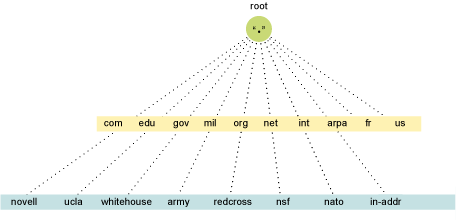
\includegraphics[width=0.6\textwidth]{img/dns.png}
    \caption{DNS hierarchy. Lower levels correspond to more specific names.}
    \label{fig:dns}
\end{figure}

For instance, in order to resolve the name \url{service.bookstore.com.}, the root node (at the top-level of the hierarchy; corresponding to the rightmost "\url{.}" of the name) is first queried in order to determine what node in the next level of the DNS hierarchy is responsible for address translation of the next part of the domain, i.e. "\url{.com}". DNS then directs the client to query this node for name-to-IP-translation recursively (usually one query for the part of the name). This process is usually repeated until the response from DNS indicates whether an IP corresponding to the queried name could be found or not.}

\end{enumerate}

\subsection{RPC Semantics}
The semantics of RPC used for \texttt{acertainbookstore.com} is ``at most
once''. This means the request from the client is at most executed once on the
server side, and if any errors occur they are exposed to the client.


\subsection{HTTP Proxy Servers}

The usual approach to using proxy servers to increase the number of simultaneous
users, is to make the proxy handle all incoming connections, and distribute the
work between ``worker'' machines (i.e.\ by round-robin).

The current setup stored the book data directly in memory, and concurrent
modifications are handled using threads, which limits the uses to a
\emph{single} (possibly multicore) machine.

In our opinion the easiest way to enable scalability would be to move the data
into a database, that every worker machine would connect to. Then we can use a
proxy server as the entry point for HTTP requests, which forwards requests to a
\texttt{BookStoreHTTPServer} on some ``worker'' machine. This of course means
the database becomes a bottleneck, but it has greatly improved the situation
from having just one machine.\footnote{and also gives you lots of features for
  handling fault tolerance for free}.

\subsection{Scalability}

As outlined above, the current setup does not facilitate running the server on
more than one machine at once, so besides upgrading the CPU to having many
cores, there is not much to do.

By employing a database, the database becomes the bottleneck. However, databases
can also be run distributed over more than one machine to improve
performance. Even though this helps, it is not a silver bullet to allow
infinitely scalability.

If a single proxy server becomes a bottleneck, one can simply add an other proxy
server in the DNS settings, so this should not be a big issue.

\subsection{Crashes}

\begin{enumerate}[(a)]
\item If the server running the \textit{CertainBookStore} class were to become
  unavailable without a proxy, a client would experience their requests timing
  out. If a proxy server is inserted between the client and the
  \textit{CertainBookStore}-server the client would receive a ``502 Bad
  Gateway'' error from the proxy instead.
\item The caching layer could be used to serve a read-only version of the
  service in case the backend-server fails. This would enable us to mask
  failures from clients only requiring read-access to the data provided by the
  service. It would, however, be unusual to employ caching proxy-servers for
  this purpose since their primary purpose is to offload repeated data accesses
  from reaching the backend servers. They usually provide no guarantee to hold a
  complete copy of the data provided by a service.
\item 
\end{enumerate}


%\bibliographystyle{plain}
%\bibliography{references}

%\section*{Appendix A}
%\subsection*{\path{src/commented-disassembly.txt}}
%\inputmintedtext}{src/commented-disassembly.txt}

%\pagebreak

%\subsection*{\path{src/exploit.c}}
%\inputminted{c}{src/exploit.c}

\end{document}

%%% Local Variables:
%%% mode: latex
%%% TeX-master: t
%%% End:
